% Figure environments for the paper's five time-trend figures.
% Requires \usepackage{graphicx} in the preamble.
% In Overleaf, place the PDF files under a folder named "figures/" (matching the
% repo layout paper/figures/*.pdf), or set \graphicspath{{figures/}} and drop the
% path prefix below. Each figure goes in the Results subsection noted above it.

% ---- Corpus overview -------------------------------------------------------
\begin{figure}[t]
  \centering
  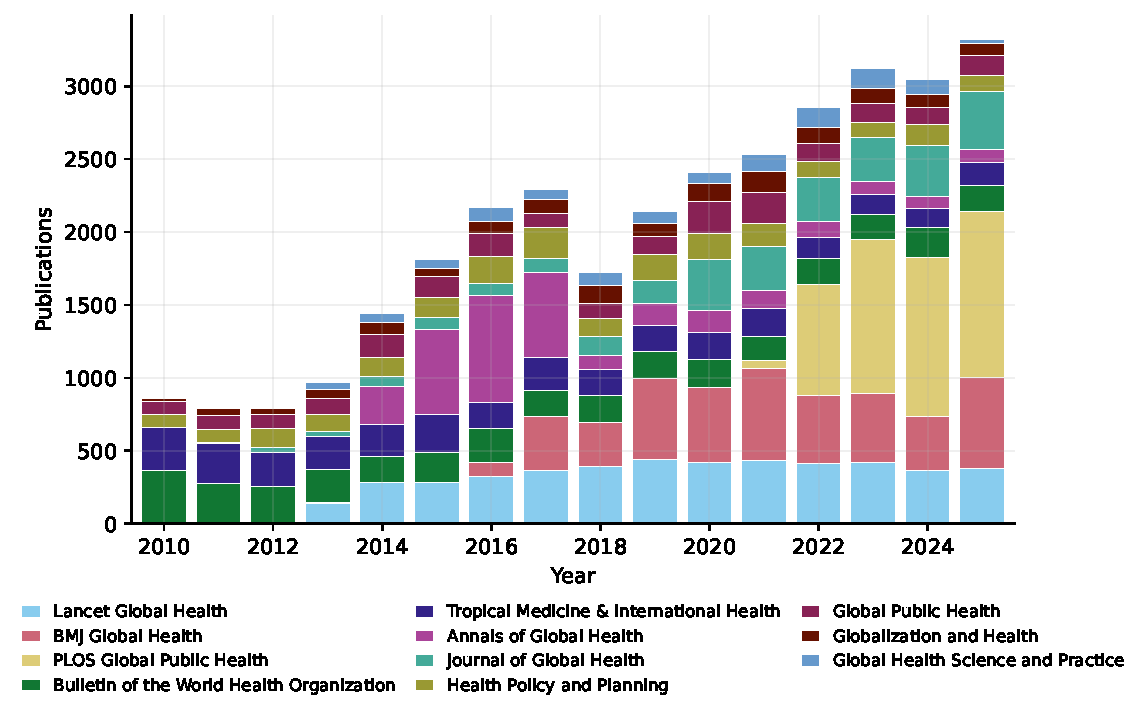
\includegraphics[width=\linewidth]{figures/fig1_publications_by_year.pdf}
  \caption{Publications by year, by journal, 2010--2025. Annual output across the
  eleven global health journals, stacked by journal. 2026 is a partial year and
  is excluded.}
  \label{fig:publications}
\end{figure}

% ---- Research funding ------------------------------------------------------
\begin{figure}[t]
  \centering
  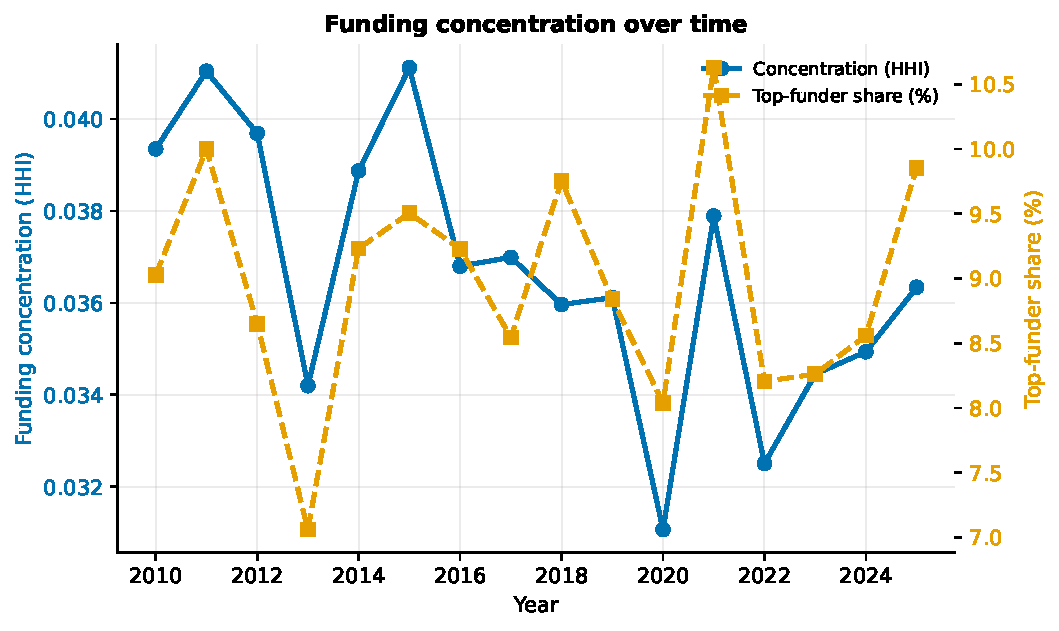
\includegraphics[width=\linewidth]{figures/fig2_funder_concentration.pdf}
  \caption{Funding concentration over time, 2010--2025. Herfindahl--Hirschman
  index of acknowledged funders per year (left axis) and the share of funded
  articles attributable to the single most frequent funder (right axis). Higher
  values indicate greater concentration.}
  \label{fig:funding}
\end{figure}

% ---- Study locations and research leadership -------------------------------
\begin{figure}[t]
  \centering
  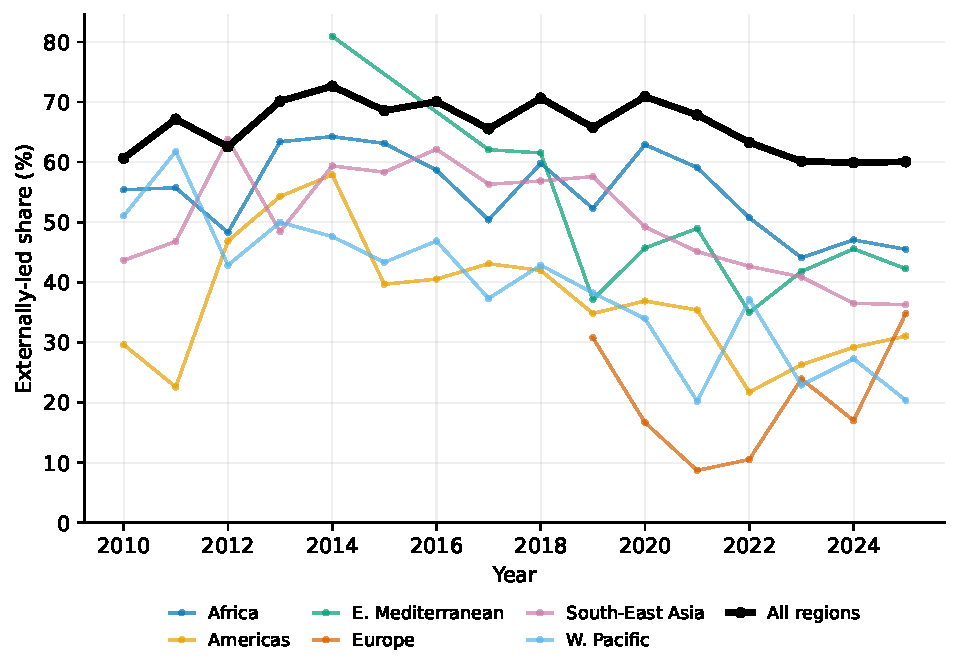
\includegraphics[width=\linewidth]{figures/fig3_externally_led.pdf}
  \caption{Externally-led (parachute) research over time, 2010--2025. Share of
  single-country research articles with no author affiliated with the study
  country, overall (black) and by WHO region (colored; region-years with fewer
  than 20 articles omitted).}
  \label{fig:externally-led}
\end{figure}

% ---- Research topics and disease burden ------------------------------------
\begin{figure}[t]
  \centering
  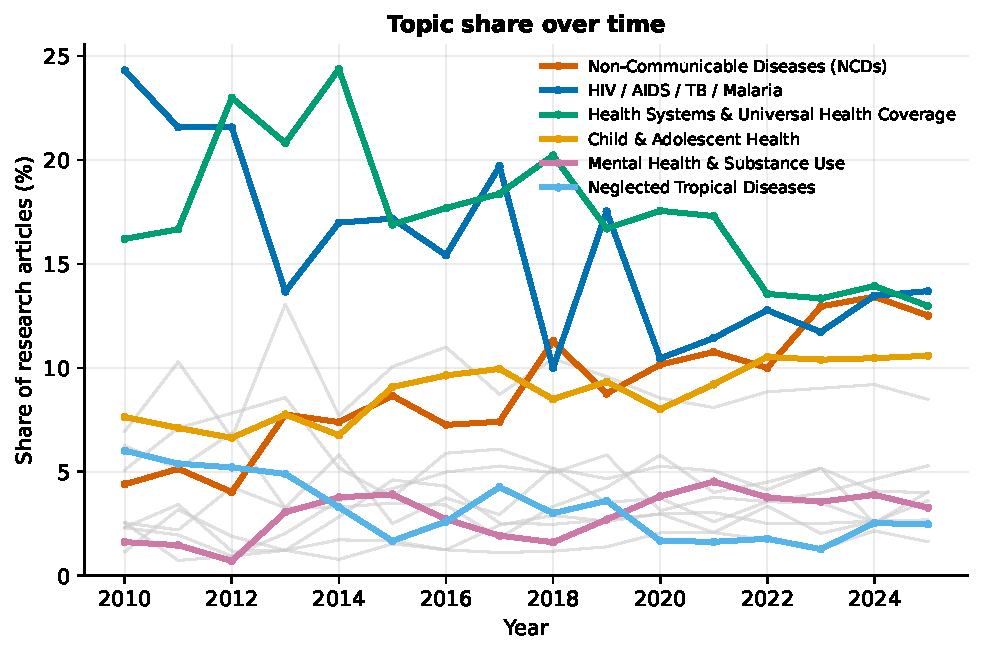
\includegraphics[width=\linewidth]{figures/fig4_topic_share.pdf}
  \caption{Topic share of research articles over time, 2010--2025. Each line is a
  primary topic's share of research articles per year; the six
  highest-movement topics are highlighted and the remaining topics are shown in
  grey.}
  \label{fig:topic-share}
\end{figure}

% ---- Producing institutions ------------------------------------------------
\begin{figure}[t]
  \centering
  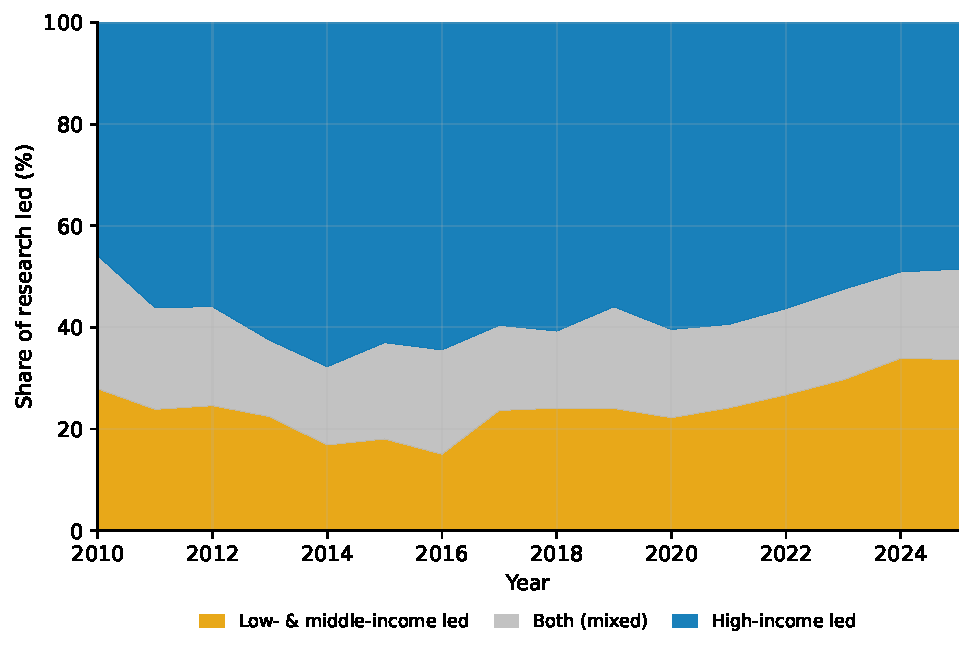
\includegraphics[width=\linewidth]{figures/fig5_north_south_leadership.pdf}
  \caption{Global North versus South research leadership over time, 2010--2025.
  Each research article is classified by the income group of its lead (first or
  last author) institutions: low- and middle-income led (all lead institutions
  in low- or middle-income countries), high-income led (all in high-income
  countries), or both. Shares are of articles with at least one lead-institution
  country.}
  \label{fig:north-south}
\end{figure}
